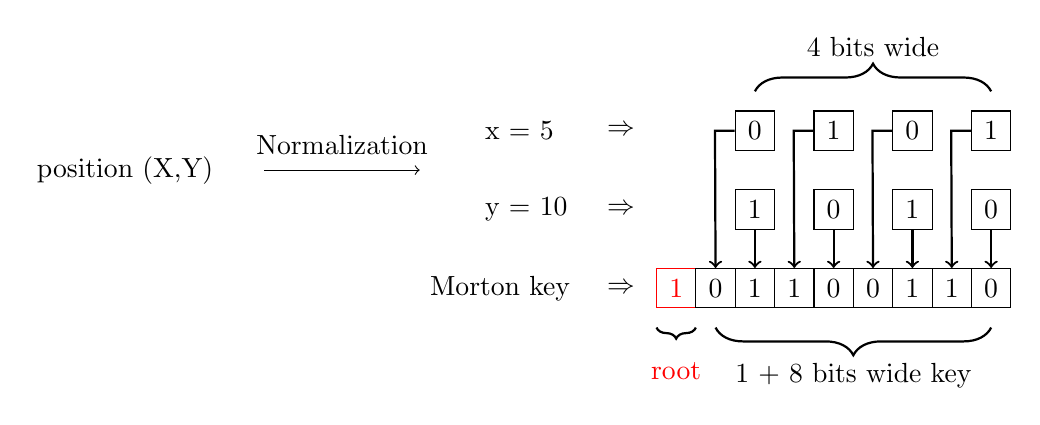
\begin{tikzpicture}

\node at (-6,4.5) (base) {position (X,Y)};
\draw[->] ([xshift=15pt]base.east) -- ([xshift=2.5cm]base.east) node[yshift=2pt,midway,above] () {Normalization};

\node[anchor=west] at (-1.55,5) {x = 5 };
\node[anchor=west] at (-1.55,4) {y = 10 };
\node[anchor=west] at (-2.25,3) {Morton key};

\node[anchor=west] at (0,5) {$\Rightarrow$};
\node[anchor=west] at (0,4) {$\Rightarrow$};
\node[anchor=west] at (0,3) {$\Rightarrow$};

\node[draw,minimum width = .5cm, minimum height = .5cm] at (2,5) (x0) {0};
\node[draw,minimum width = .5cm, minimum height = .5cm] at (3,5) (x1) {1};
\node[draw,minimum width = .5cm, minimum height = .5cm] at (4,5) (x2) {0};
\node[draw,minimum width = .5cm, minimum height = .5cm] at (5,5) (x3) {1};

\node[draw,minimum width = .5cm, minimum height = .5cm] at (2,4) (y0) {1};
\node[draw,minimum width = .5cm, minimum height = .5cm] at (3,4) (y1) {0};
\node[draw,minimum width = .5cm, minimum height = .5cm] at (4,4) (y2) {1};
\node[draw,minimum width = .5cm, minimum height = .5cm] at (5,4) (y3) {0};

% Result
\node[draw,minimum width = .5cm, minimum height = .5cm,red] at (1,3) (root) {1};
%\node[red] at ([yshift=-10pt]root.south) {root};

\node[draw,minimum width = .5cm, minimum height = .5cm] at (1.5,3) (k0) {0};
\node[draw,minimum width = .5cm, minimum height = .5cm] at (2,3) (k1) {1};
\node[draw,minimum width = .5cm, minimum height = .5cm] at (2.5,3) (k2) {1};
\node[draw,minimum width = .5cm, minimum height = .5cm] at (3,3) (k3) {0};
\node[draw,minimum width = .5cm, minimum height = .5cm] at (3.5,3) (k4) {0};
\node[draw,minimum width = .5cm, minimum height = .5cm] at (4,3) (k5) {1};
\node[draw,minimum width = .5cm, minimum height = .5cm] at (4.5,3) (k6) {1};
\node[draw,minimum width = .5cm, minimum height = .5cm] at (5,3) (k7) {0};

\draw [thick,decorate,decoration={brace,amplitude=4pt}]
(1.25,2.5) -- (.75,2.5)  node [red,midway,below,yshift=-9pt] 
{root};

\draw [thick,decorate,decoration={brace,amplitude=10pt}]
(5,2.5) -- (1.5,2.5)  node [midway,below,yshift=-9pt] 
{1 + 8 bits wide key};

\draw [thick,decorate,decoration={brace,amplitude=10pt}]
(2,5.5) -- (5,5.5)  node [midway,above,yshift=9pt] 
{4 bits wide};

% Arrows
\draw[thick,->] (y3.south) -- (k7.north);
\draw[thick,->] (y2.south) -- (k5.north);
\draw[thick,->] (y1.south) -- (k3.north);
\draw[thick,->] (y0.south) -- (k1.north);

\draw[thick,->] (x3.west) -- ([xshift=-.25cm]x3.west) -- (k6.north);
\draw[thick,->] (x2.west) -- ([xshift=-.25cm]x2.west) -- (k4.north);
\draw[thick,->] (x1.west) -- ([xshift=-.25cm]x1.west) -- (k2.north);
\draw[thick,->] (x0.west) -- ([xshift=-.25cm]x0.west) -- (k0.north);
%\draw[thick,->] (y2.west) -- (k5.north);
%\draw[thick,->] (y1.west) -- (k3.north);
%\draw[thick,->] (y0.west) -- (k1.north);
\end{tikzpicture}